\chapter{Computação em Nuvem}

Com o rápido desenvolvimento das tecnologias de processamento e de armazenamento, recursos computacionais ficaram mais baratos, mais poderosos e mais ubiquoamente disponíveis. Esta tendência tecnológica permitiu a realização de um novo modelo computacional chamado Computação em Nuvem, no qual recursos são oferecidos como serviços de utilidade geral que podem ser alocados e desalocados por usuários pela internet sob demanda. A emerção da Computação em Nuvem causou um grande impacto nas industrias de tecnologia da informação nos últimos anos, onde grandes empresas como Google, Amazon e Miscrosoft rivalizam para prover plataformas de nuvem mais potentes, confiáveis e economicamente eficientes, enquanto que as empresas de negócios procuram adequar seus modelos de negócio para ganhar beneficios desse novo paradigma.

Apesar do atual destaque à Computação em Nuvem,
 seu conceito não é novo e tão pouco suas
tecnologias~\cite{CloudUncovered:2012}. Em 1960 John McCarthy acreditava que um dia corporações conseguiriam vender recursos computacionais como ``commodity''~\cite{demystifingCloud:2011}.

O objetivo deste capítulo é fazer um estudo sobre a Computação em Nuvem, suas características, definições, desafios e arquitetura. Ele é dividido em 6 seções. Na primeira~\ref{cloud:def} seção são apresentados as
principais definições de computação em nuvem. Na segunda~\ref{cloud:char} seção são
apresentadas suas principais características. Na terceira~\ref{cloud:bus} seção, os modelos de
negócio possibilitados pela nuvem são explicados. Na quarta~\ref{cloud:arch} seção é feita uma
análise da arquitetura da nuvem. Na quinta~\ref{cloud:types} seção é feita uma revisão dos os
tipos de nuvem. Por fim, na sexta~\ref{cloud:chal} seção os principais desafios da área são
apresentados.

%%%%%%%%%%%%%%%%%%%%%%%%%%%%%%%%%%%%%
\section{Definição} \label{cloud:def}
%%%%%%%%%%%%%%%%%%%%%%%%%%%%%%%%%%%%%

A Nuvem já foi definida de várias formas diferentes. Em
\cite{CloudDefinition:2009}, 22  definições diferentes de Nuvem são estudadas e, a partir dessas definições, é proposta uma nova definição que contempla as demais:
	
	\begin{quotation}
		``Clouds are a large pool of easily usable and accessible virtualized resources (such as hardware, development platforms and/or services). These resources can be dynamically reconfigured to adjust to a variable load (scale), allowing also for an optimum resource utilization. This pool of resources is typically exploited by a pay-per-use model in which guarantees are offered by the Infrastructure Provider by means of customized SLAs (Service-level agreements).''
	\end{quotation}
	
	A NIST (National Institute of Standards and Technology) em ``The NIST Definition of Cloud Computing''~\citeyearpar{NIST:2011} define a Computação em Nuvem abaixo:
	
	\begin{quotation}
		``Cloud Computing is a model for enabling ubiquitous, convenient, on-demand network access to a shared pool of configurable computing resources (e. g., networks, servers,             storage, applications and services) that can be rapidly provisioned and released with minimal management effort or service provider interaction. This cloud model is composed of five essential characteristics, three service models and four deployment models.''
	\end{quotation}	
	
	As cinco características essenciais, os três modelos de serviço e os quatro tipos de nuvem citados acima são descritas nas seções seguintes.		

%%%%%%%%%%%%%%%%%%%%%%%%%%%%%%%%%%%%%
\section{Características} \label{cloud:char}
%%%%%%%%%%%%%%%%%%%%%%%%%%%%%%%%%%%%%
	Em ``The NIST Definition of Cloud Computing''~\citeyearpar{NIST:2011} é definido que a Computação em Nuvem é composta de cinco características essenciais. Essas características são descritas abaixo:   

\begin{description}

	\item[Autoatendimento sob demanda:] Um cliente da nuvem pode alocar recursos como processamento e armazenamento, sem que para isso seja necessário qualquer interação humana.
	
	\item[Amplo acesso a rede:] Os recursos da nuvem devem estar disponíveis através de uma rede (Internet, por exemplo) e podem ser acessados por mecanismos que permitam o acesso por uma gama heterogênea de plataformas como celulares, tablets e notebooks.
	
	\item[\textit{Pooling} de recursos:] Os recursos computacionais do provedor estão agrupados para servir a múltiplos consumidores, utilizando um modelo \textit{multi-tenancy}, onde diferentes recursos físicos e virtuais são dinamicamente alocados e desalocados de acordo com a demanda do consumidor. Existe um senso de independência de localização que significa que o consumidor não tem controle nem conhecimento da localização exata dos recursos alocados.
	
	\item[Elasticidade rápida:] Os recursos podem ser elasticamente provisionados, ou seja, quando é necessário mais recursos eles são alocados de forma automática e quando desnecessários esses recursos são desalocados, dando a ideia de que os recursos são ilimitados.
	
	\item[Serviços mensurados:] A nuvem deve ter a capacidade de controlar e otimizar a utilização dos recursos. Dessa forma a utilização dos recursos pode ser monitorada, controlada e reportada, tornando seu  uso transparente tanto para o provedor quanto para o consumidor.

\end{description} 



%%%%%%%%%%%%%%%%%%%%%%%%%%%%%%%%%%%%%
\section{Modelo de Negócio} \label{cloud:bus}
%%%%%%%%%%%%%%%%%%%%%%%%%%%%%%%%%%%%%

A computação em nuvem implementa um modelo de negócio orientado a serviços. Em outras palavras, os recursos de hardware e recursos a nível de plataforma são oferecidos como serviços sob demanda. De acordo com Zhang et al.~\citeyearpar{stateOfArt:2010} os serviços oferecidos pelas nuvens podem ser agrupados em três categorias: \textit{Infrastructure as a Service} (IaaS), \textit{Platform as a Service} (PaaS) e \textit{Software as a Service} (SaaS).

\begin{description}

\item[\textit{Infrastructure as a Service}:] IaaS refere-se ao provisionamento sob demanda dos recursos de infraestrutura, normalmente máquinas virtuais (\textit{virtual machines}, VMs). O dono de uma nuvem que oferece IaaS é chamado de provedor IaaS. Amazon EC2~\cite{AmazonEC2:Online}, GoGrid~\cite{GoGrid:Online} e FlexiScale~\citep{Aguiar:2005} e~\cite{FlexiScale:Online} são exemplos de provedores IaaS.

\item [\textit{Platform as a Service}:] PaaS refere-se ao provisionamento de recursos de plataforma, como sistemas operacionais e frameworks de desenvolvimento de software. Exemplos de provedores PaaS são: Google App Engine~\cite{GoogleAppEngine:Online}, Microsoft Windows Azure~\cite{MicrosoftAzure:Online} e Salesforce~\cite{Salesforce:Online}.

\item[\textit{Software as a Service}:] SaaS refere-se ao provisionamento de aplicações sob demanda. Exemplos de provedores SaaS incluem: Rackspace~\cite{Rackspace:Online} e SAP Business By Design~\cite{SAP:Online}.

\end{description}

O modelo de negócio da computação em nuvem é apresentado na Figura \ref{business-model}. De acordo com a arquitetura em camadas da nuvem é possível que um provedor PaaS funcione sobre um provedor IaaS. Porém o que é muito comum atualmente é que a mesma organização seja o provedor PaaS e IaaS, como a Google e a SalesForce.com. Por esse motivo, provedores PaaS e IaaS são frequentemente chamados de provedores de infraestrutura ou provedores de nuvem.

\begin{figure}[htbp]
  \centering 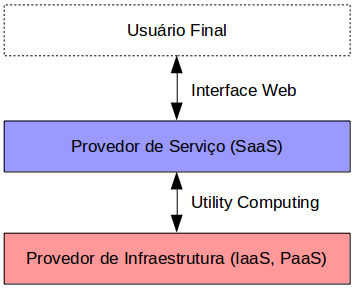
\includegraphics[scale=.6]{imgs/business-model.png}
\caption{Modelo de negócio da computação em nuvem.} 
\label{business-model}
\end{figure}


%%%%%%%%%%%%%%%%%%%%%%%%%%%%%%%%%%%%%
\section{Arquitetura} \label{cloud:arch}
%%%%%%%%%%%%%%%%%%%%%%%%%%%%%%%%%%%%%

Para Zhang et al.\citeyearpar{stateOfArt:2010} a arquitetura da computação em Nuvem é divida em quatro camadas: a camada de hardware, a camada de infraestrutura, a camada de plataforma e a camada de aplicação, como apresentado na Figura \ref{architecture1}. As camadas são detalhadas abaixo:

\begin{figure}[htbp]
  \centering 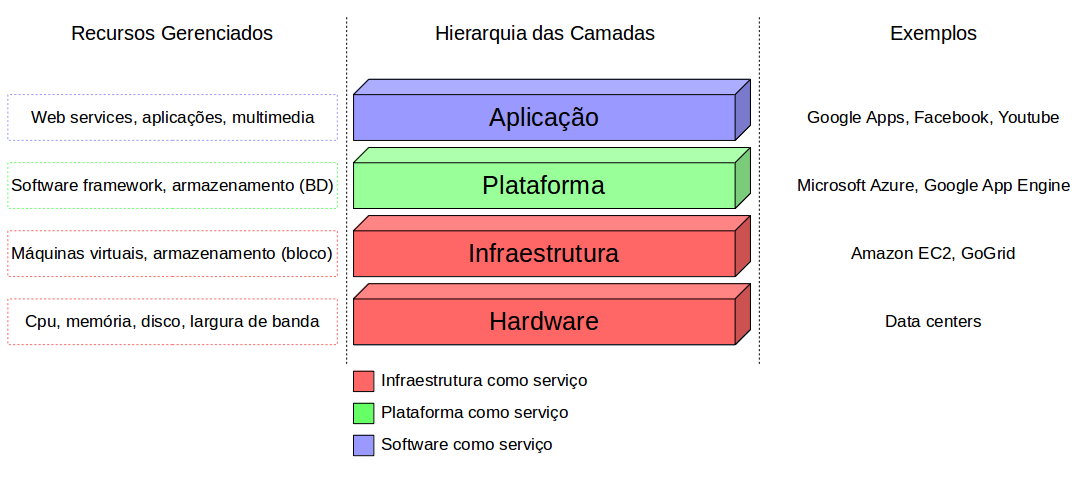
\includegraphics[scale=.4]{imgs/architecture1.png}
\caption{Arquitetura da Computação em Nuvem segundo~\citep{stateOfArt:2010}} 
\label{architecture1}
\end{figure}

\begin{description}

	\item[Camada de Hardware:] essa camada é responsável pela gestão dos recursos físicos, incluindo servidores, roteadores, switches, sistemas de resfriamento e energia. Na prática, a camada de      hardware é tipicamente implementada nos data centers. Um data center normalmente contém milhares de servidores organizados em racks e interconectados através de switches ou roteadores. Problemas típicos na camada de hardware envolvem configuração de hardware, tolerância a falhas, gerenciamento do tráfego, gerenciamento de energia e gerenciamento dos recursos de resfriamento.

	\item[Camada de Infraestrutura:] também conhecida como camada de virtualização, a camada de infraestrutura cria uma pool de armazenamento e recursos computacionais através do particionamento dos recursos físicos utilizando tecnologias de virtualização como  Xen~\cite{Xen:Online}, KVM~\cite{KVM:Online} e VMware~\cite{VMware:Online}. Como as principais características da computação em nuvem, como alocação dinâmica de recursos, só são possíveis por causa das tecnologias de virtualização, a camada de infraestrutura é considerada um componente essencial na arquitetura.

	\item[Camada de Plataforma:] construída sobre a camada de infraestrutura, a camada de plataforma consiste em sistemas operacionais e frameworks. O propósito da camada de plataforma é facilitar o lançamento de aplicações em máquinas virtuais. Por exemplo, o Google App Engine opera na camada de plataforma provendo uma API com suporte para armazenamento e lógica de negócio para aplicações web típicas. 

	\item[Camada de Aplicação:] no nível mais alto da hierarquia, a camada de aplicação consiste nas aplicações da nuvem. Diferentes das aplicações tradicionais, as aplicações da nuvem fazem uso do escalonamento automático disponível na Nuvem para alcançar um melhor desempenho, disponibilidade e baixo custo de operação.

\end{description}

Comparado aos ambientes de hospedagem de serviços tradicionais como servidores dedicados, a arquitetura da nuvem é mais modular. Cada camada é fracamente acoplada, com camadas acima e abaixo, permitindo que cada camada evolua separadamente. Essa modularidade permite que a computação em nuvem dê suporte a uma gama de requerimentos das aplicações enquanto reduz o sobrecusto de manutenção e de administração.

Para Hassan et al.~\citeyearpar{demystifingCloud:2011} a arquitetura também é dividida em quatro camadas com uma hierarquia baseada na abstração, porém a arquitetura é definida diretamente ligada aos modelos de negócio, como pode ser observado na Figura \ref{architecture2}. Nessa definição é adicionando um novo modelo de negócio: dados como serviço, que é descrito como o serviço que oferece base de dados para armazenamento das informações do cliente. 

\begin{figure}[htbp]
  \centering 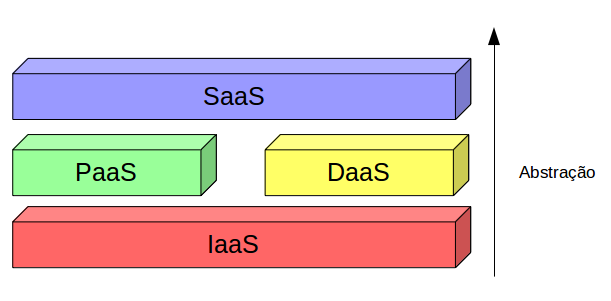
\includegraphics[scale=.6]{imgs/architecture2.png}
\caption{Arquitetura da Computação em Nuvem segundo~\citep{demystifingCloud:2011}} 
\label{architecture2}
\end{figure}

%%%%%%%%%%%%%%%%%%%%%%%%%%%%%%%%%%%%%
\section{Tipos de Nuvem} \label{cloud:types}
%%%%%%%%%%%%%%%%%%%%%%%%%%%%%%%%%%%%%

	Zhang et al.~\citeyearpar{stateOfArt:2010} e Mell et al.~\citeyearpar{NIST:2011} descrevem 4 tipos de nuvem: Nuvem Pública, Nuvem Privada, Nuvem Híbrida e Nuvem Comunitária.

	\begin{description}
	
		\item[Nuvem Pública:] nuvem onde os provedores de serviços oferecem seus recursos ao público geral. Nuvens públicas oferecem vários benefícios aos provedores de serviço: por exemplo, não é necessário para os provedores investimentos inciais em infraestrutura. No entanto, as nuvens públicas oferecem um baixo grau de controle sobre os dados, a rede e as configurações de segurança.  	 
			
		\item[Nuvem Privada:] também conhecida como nuvem interna, as nuvens privadas são para uso exclusivo de uma organização. A nuvem privada pode ser construída e gerenciada pela própria empresa ou por provedores externos. Esse tipo de nuvem oferece um maior controle de desempenho, segurança e confiabilidade. No entanto, as nuvens privadas são criticadas por serem muito similares aos servidores tradicionais.
		
		\item[Nuvem Híbrida:] uma nuvem híbrida é a combinação da nuvem privada e da nuvem pública, na tentativa de minimizar as limitações das duas abordagens. Nesse tipo de nuvem, parte dos serviços de infraestrutura estão na nuvem privada enquanto que as outras partes são executadas em uma nuvem pública. Nuvens híbridas oferecem mais flexibilidade que as nuvens públicas e do que as nuvens privadas. Elas oferecem mais controle sobre dados, rede e segurança do que as nuvens públicas mantendo as facilidades de expansão.
		
		\item[Nuvem Comunitária:] a nuvem comunitária funciona praticamente como uma nuvem privada que pode ser utilizada por duas ou mais organizações. Ela pode ser gerenciada tanto por uma organização, pelas duas organizações, ou por um provedor.
		 	
	\end{description}
	
%%%%%%%%%%%%%%%%%%%%%%%%%%%%%%%%%%%%%
\section{Desafios} \label{cloud:chal}
%%%%%%%%%%%%%%%%%%%%%%%%%%%%%%%%%%%%%

	Apesar da Computação em Nuvem estar amplamente presente na indústria, as pesquisas nessa área ainda estão em fase inicial~\cite{stateOfArt:2010}.  Muitos problemas existentes ainda não foram resolvidos, enquanto novos desafios continuam surgindo das aplicações nas indústrias. Esta seção apresenta um resumo dos principais desafios da Computação em Nuvem. 
	
	\subsection{Provisionamento Automático de Serviço}
	Umas das principais características da Computação em Nuvem é a capacidade de adquirir e liberar recursos sob demanda. O objetivo de um provedor de serviço neste caso é de alocar e desalocar recursos da nuvem a fim de satisfazer os service nível objectives (SLOs), enquanto minimiza o custo operacional.  No entanto, não é óbvio como o provedor de serviço alcançará esse objetivo. Em particular, não é fácil de determinar como mapear SLOs tais como requisitos de QoS para requisitos dos recursos de baixo nível como requisitos de CPU e de memória. Além disso, para alcançar alta agilidade para responder as flutuações de demanda, as decisões de provisionamento devem ser feitas em tempo real.
	
	\subsection{Migração de Máquinas Virtuais}
	A virtualização é uma das principais tecnologias utilizadas em infraestruturas em nuvem. Através do uso da virtualização, é possível compartilhar a mesma máquina física com múltiplos sistemas operacionais e/ou aplicações de usuários finais, promovendo o isolamento entre os mesmos. Da mesma forma, o seu uso torna possível realizar balanceamento de carga entre estruturas físicas, através de ações como a migração de máquinas virtuais entre servidores.
	
	A migração de VMs evoluiu das técnicas de migração de processos~\cite{Osman:2002}. Algumas ferramentas já implementam o conceito de live-migration, onde as VMs são movidas em um processo que envolve paradas extremamente curtas que variam de dezenas de milissegundos a um segundo. Clark et al.~\citeyearpar{Clark:2005} mostra que a migração de um SO inteiro e todas suas aplicações como uma unidade permite que muitas das dificuldades encontradas nas abordagens de migração de processos sejam evitadas.
	 
	O maior benefício da migração de VMs é a capacidade de evitar a sobrecarga de pontos específicos da infraestrutura de servidores. No entanto, essa não é uma tarefa simples. Atualmente, a detecção de pontos de sobrecarga e o disparo de uma migração não tem agilidade suficiente para responder às mudanças de carga de trabalho repentinas~\cite{stateOfArt:2010}. Além disso, é necessário transferir o estado dos dados em memória de forma consistente e eficiente, considerando os recursos para as aplicações e para os servidores físicos.
	
	\subsection{Consolidação de Servidores}
	A consolidação de servidores é uma abordagem que tem como objetivo maximizar a utilização de recursos enquanto minimiza o consumo de energia. A técnica de migração de VMs é frequentemente utilizada na consolidação de servidores, onde VMs são movidas de múltiplos servidores subutilizados para um servidor. Dessa forma os servidores restantes são colocados no estado de economia de energia. O problema de consolidar servidores de forma ótima pode ser visto como uma variação do problema bin-packing~\cite{Chekuri:1999}, que é um problema de otimização NP-difícil.
	
	\subsection{Gerenciamento de Energia}
	Atingir uma maior eficiência no consumo de energia também é um dos principais desafios da computação em nuvem. Hamilton et al.~\citeyearpar{Hamilton} estima que o custo de alimentação energética e refrigeração somam 53 por cento dos gastos operacionais dos data centers. Em 2006, os data centers nos Estados Unidos consumiram mais de 1.5 porcento de toda energia gerada naquele ano, e o crescimento dessa porcentagem tem projeção de crescimento de 18 porcento ao ano. Isso leva a uma enorme pressão sobre os provedores de infraestrutura para a redução do consumo energético. O objetivo não é apenas reduzir o gasto energético, mas também se adequar aos regulamentos do governo e as normas ambientais. 
	
	\subsection{Segurança dos Dados}
	A segurança dos dados é outro tópico de pesquisa muito importante na computação em nuvem. Visto que os provedores dos serviços tipicamente não têm acesso aos sistemas de segurança dos data centers, eles dependem do provedor de infraestrutura para garantir a segurança de seus dados. Os provedores de infraestrutura devem garantir:
	\begin{description}
		\item[Confidencialidade] para garantir a segurança de acesso e transferência de dados.
                   
		\item[Auditabilidade] para atestar se as configurações de segurança de uma aplicação foram modificadas ou não.  
	\end{description}	 
	
	Confidencialidade é normalmente alcançada utilizando protocolos de criptografia, enquanto que a auditabilidade é alcançada utilizando técnicas de atestado remoto. Atestados remotos tipicamente necessitam de um trusted platform module (TPM) para gerar um sumário do sistema infalsificável como prova da segurança do sistema. Porém num ambiente como a nuvem onde as VMs podem migrar dinamicamente de um servidor para outro, utilizar atestado remoto não é o suficiente. É necessário que seja criado um mecanismo confiável em cada camada da arquitetura. Inicialmente, para ser confiável, a camada de hardware deve usar um TPM. A camada de infraestrutura, responsável pela migração das VMs, deve utilizar monitores de VMs confiáveis. A migração de VMs só deve ser permitida se tanto o servidor de destino quanto fonte são confiáveis.


